\documentclass[14pt]{matmex-diploma}
\usepackage{tikz}
\usepackage{pgfplots}
\pgfplotsset{compat=1.9}
\begin{document}
\filltitle{ru}{
    chair              = {Кафедра системного программирования},
    title              = {Поддержка конъюнктивных грамматик в GLL},
    type               = {coursework},
    position           = {студента},
    group              = 371,
    author             = {Горохов Артем Владимирович},
    supervisorPosition = {магистр ИТ, ст. преп.},
    supervisor         = {Григорьев С.\,В.}
}
\maketitle
\tableofcontents


\section*{Аннотация}

В работе представлена модернизация реализации алгортма синтаксического анализа регулярных мнрожеств, основанного на алгоритме синтаксического анализа GLL. Модернизация позволяет расширить класс распознаваемых анализатором языков до конъюнктивных, что полезно в некоторых задачах, например синтаксический анализ метагеномных сборок.

\section*{Введение}

Синтаксический анализ, как правило, используется для построения структурного представления кода с использованием грамматики, описывающей разбираемый язык. Абстрактное синтаксическое дерево, являющееся результатом работы синтаксического анализатора, в дальнейшем используется для проведения статического анализа кода или же в каких-то других целях. Как правило, на вход синтаксическому анализатору подаётся линейная последовательность токенов, представляющая код программы. Однако могут возникать ситуации, когда вход не может быть представлен линейно. Такие ситуации могут возникать, например, при автоматической генерации кода. Генерация может происходить в циклах, с использованием условных операторов или строковых операций. Поэтому для описания генерируемых цепочек можно использовать конечный автомат, порождающий цепочки, который уже не будет являться линейным. Такую задачу будем называть синтаксическим анализом регулярных множеств.

Кроме этого, ещё одной областью, где может быть применим синтаксический анализ регулярных множеств является бионформатика. Одной из часто возникающих задач в биоинформатике является классификация организмов, находящихся в образцах, полученных из окружающей среды~\cite{bioRNA}. По образцам строится метагеномная сборка, которая содержит в себе смесь из РНК всех содержащихся в сборке организмов. В свою очередь РНК является последовательностью символов в алфавите \{A, C, G, T\}. РНК организмов, которые относятся к одному и тому же виду, содержат одинаковые подцепочки, которые и необходимо выделить, чтобы классифицировать организм. Как правило, эти подцепочки --- это последовательности РНК. РНК может быть описана с помощью грамматики. Метагеномная сборка, в свою очередь, может быть представлена в виде графа с цепочками на рёбрах. Таким образом, в таком графе необходимо найти цепочки, выводимые в грамматике, описывающей РНК. 

Грамматики, описывающие структуру РНК, являются неоднозначными. Грамматика называется неоднозначной, если одна и та же цепочка может быть выведена несколькими способами. Такие алгоритмы синтаксического анализа как LR и LL не позволяют обрабатывать неоднозначные грамматики. Для работы с неоднозначными грамматиками существуют алгоритмы обобщённого синтаксического анализа GLR~\cite{GLR}, GLL~\cite{GLL}. В рамках проекта YaccConstructor~\cite{YaccConstructorPage, YaccConstructorPaper} был реализован алгоритм GLL, кроме того, была предложена его модификация для обработки нелинейных входных данных --- графов. Реализованная модификация позволяет находить цепочки транспортной РНК(тРНК) в небольших метагеномных сборках, возвращая координаты начала и конца найденной цепочки. Проблема заключается в том, что грамматика для описания тРНК является сильно неоднозначной, что сказывается на производительности и точности полученных результатов. Для повышения точности можно применять конъюнктивные грамматики~\cite{ConjGrammars}, в которых для описания продукций используется операция конъюнкции. Такие грамматики расширяют класс контекстно-свободных языков и позволяют точнее описать структуру тРНК. Данная работа посвящена описанию модификаций решения на основе алгоритма GLL для работы с конъюнктивными грамматиками.

\section{Обзор предметной области}
Одной из задач, часто возникающих в биоинформатике, является классификация организмов в образцах, полученных из окружающей среды. Из образцов извлекается смесь РНК всех организмов, которая представляется в виде метагеномнонй сборки. Метагеномная сборка, в свою очередь, может быть представлена в виде конечного автомата, порождающего геномы всех организмов из образца. Для того, чтобы определить, к какому виду относится организм, нужно выделить РНК. Для поиска РНК в метагеномных сборках существуют различные подходы. Некоторые из них используют скрытые модели Маркова~\cite{markov} для поиска, например, инструмент REAGO~\cite{REAGO}. Минусом инструмента является то, что он не работает с метагеномной сборкой, представленной в виде графа, а представление сборки в другом виде требует слишком больших объёмов памяти. Инструмент Xander~\cite{Xander} позволяет работать со сборками, представленными в виде графов, но в основе лежит механизм, обладающий низкой точностью. Синтаксический анализ, также, применяется для анализа метагеномных сборок, например, в инструменте Infernal~\cite{Infernal}, который не предназначен для работы с графами.

Грамматика, описывающая РНК является сильно неоднозначной и её не всегда можно привести к однозначной форме. Для работы с неоднозначными грамматиками используются алгоритмы обобщённого синтаксического анализа. Принцип работы таких алгоритмов заключается в том, что они просматривают все возможные пути вывода входной цепочки и строят все деревья вывода этой цепочки. Существует инструмент SBP~\cite{SBP} основанный на алгоритме GLR, позволяющий работать с конъюнтивными грамматиками. В данной работе используется алгоритм GLL, так как в среднем он работает быстрее. Алгоритм обобщённого анализа GLL основан на нисходящем анализе и отличается высокой скоростью работы и простотой. В алгоритме для хранения всех деревьев вывода используется структура данных SPPF (Shared Packed Parse Forest)~\cite{SPPF}. Эта структура данных позволяет переиспользовать узлы, с одинаковыми поддеревьями под ними. На рисунке~\ref{SPPF} показано, как объединяются разные выводы нетерминала $ S $. Создаются дополнительные узлы, соответствующие каждому из выводов. Выделяются одинаковые поддеревья и остаётся только один экземпляр каждого, на который, в дальнейшем, ссылаются предки.

\begin{figure}
\centering
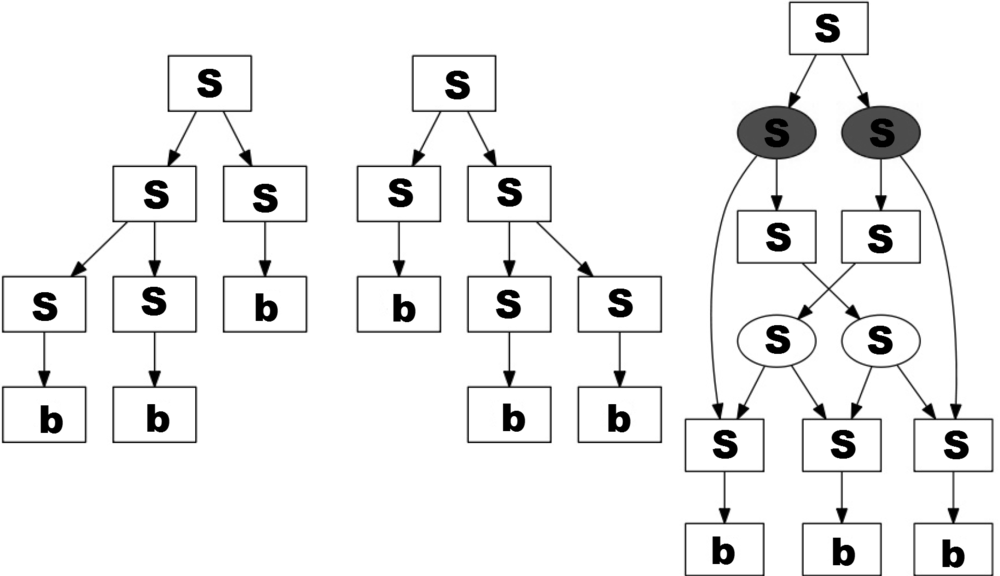
\includegraphics[width=14cm]{courseworkpictures/SPPF.PNG}
\caption{Преобразование дерева разбора к SPPF}
\label{SPPF}
\end{figure}

\begin{figure}
$$
\begin{array}{crcl}
& \mbox{\texttt{ S }} &::=& \mbox{\texttt{ A B }} \& \mbox{\texttt{ D C}} \\
& \mbox{\texttt{ A }} & ::=& \mbox{\texttt{ a A |}}  \epsilon \\
& \mbox{\texttt{ B }} & ::=& \mbox{\texttt{ b B c |}}  \epsilon \\
& \mbox{\texttt{ C }} & ::=& \mbox{\texttt{ c C |}}  \epsilon \\
& \mbox{\texttt{ D }} & ::=& \mbox{\texttt{ a D b |}}\epsilon \\
\end{array}
$$
\caption{Грамматика для контекстно-зависимого языка \{$a^n b^n c^n, n \geq 0$\}}
\label{gabc}
\end{figure}

Алгоритм GLL позволяет работать с любыми КС-грамматиками, в том числе и сильно неоднозначными. Однако наличие сильной неоднозначности в грамматике сказывается на точности получаемых результатов и производительности. 
  Конъюнктивные грамматики при описании правил вывода используют операцию конъюнкции. Цепочка принадлежит языку, задаваемому такой грамматикой, если существует вывод по обоим конъюнктам. На рисунке~\ref{gabc} изображена грамматика для языка не являющегося контекстно-свободным, описанная с помощью операции конъюнкции. Такие грамматики дают возможность точно описать структуру тРНК, что позволяет снизить количество ошибок при разборе.

\section{Постановка задачи}

Целью данной работы является добавление поддержки конъюнктивных грамматик в YассConstructor. Для её достижения были поставлены следующие задачи:

\begin{itemize}
    \item реализовать поддержку конъюнктивных грамматик в языке спецификации грамматик YARD;
    \item реализовать поддержку конъюнктивных грамматик в генераторе GLL-анализаторов;
    \item провести экспериментальные исследования работы алгоритма.
\end{itemize}


\section{Основная часть}

В данном разделе рассмотреннно расширение языка YARD и модификация алгоритма синтаксического анализа GLL.


\subsection{Архитектура}

Ввиду модульной структуры проекта YaccConstructor, задействованную структуру проекта можно разделить на части, показанные на рисунке~\ref{project_structure}.

В проекте используется язык описания грамматик YARD~\cite{YARD}, который поддерживает различные конструкции, упрощающие разработку грамматик: повторения \verb|x*[1..10]|, дизъюнкции \texttt{A|B}, условное вхождние и подобные. Перед подачей генератору, дерево разбора грамматики проходит через множество преобразований, в результате которых, грамматика приводится к форме Бэкуса-Наура~\cite{BNF}.

\begin{figure}[h]
\centering
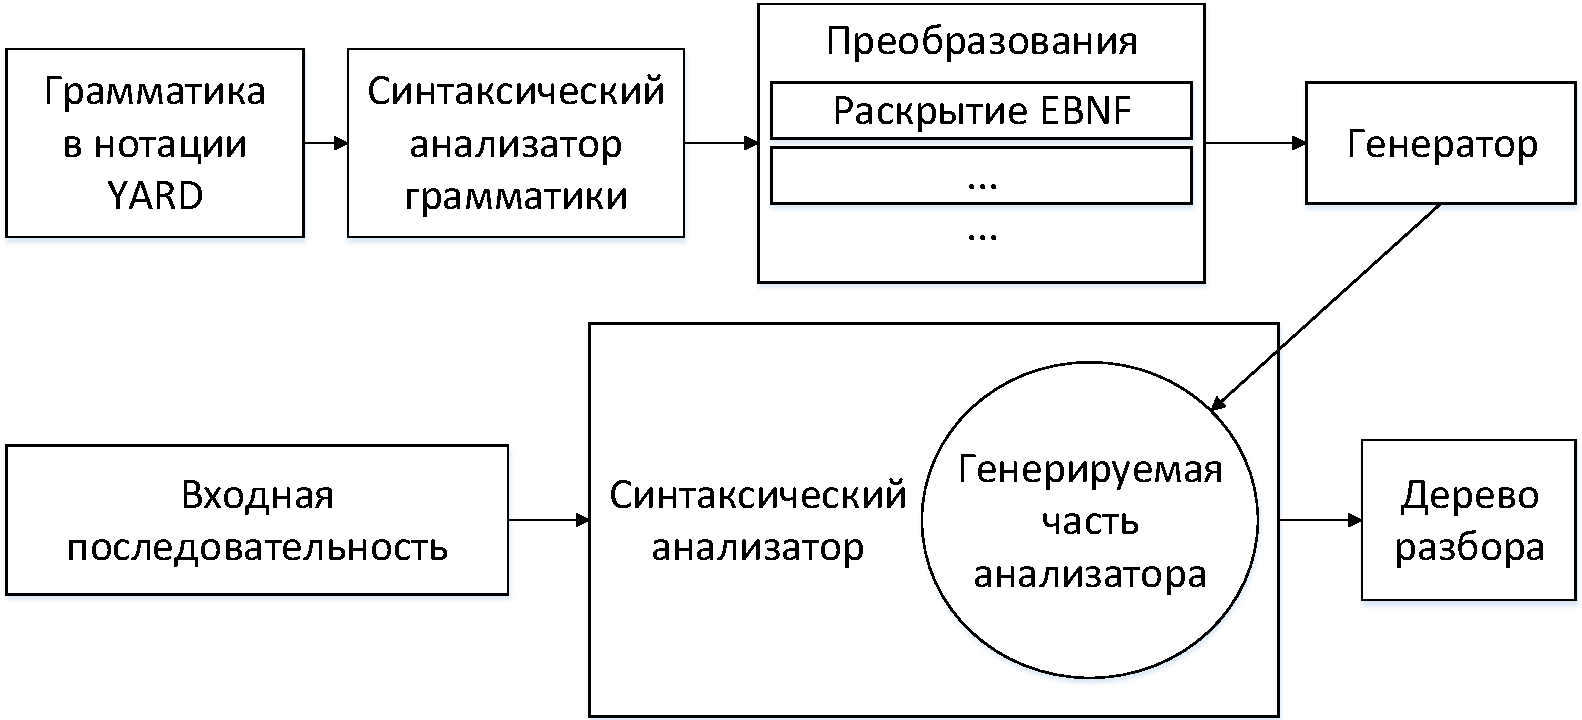
\includegraphics[width=15cm]{courseworkpictures/img2.pdf}
\caption{Структура существующего решения}
\label{project_structure}
\end{figure}

\subsection{Расширение YARD}
Для работы с конъюнктивными грамматиками в язык YARD была добавлена новая конструкция: конъюнкция, приоритет которой между дизъюнкцией и последовательностью. Язык YARD поддерживает различные конструкции вроде повторений (x*[1..10]), которые преобразуются перед подачей генератору. Так как в язык была добавлена новая конструкция, нужно было обеспечить её поддержку во всех существующих преобразованиях.

Кроме того, добавленную конструкцию также необходимо преобразовывать к виду, принимаемому генератором. Предлагается следующее решение: грамматика преобразовывается к контекстно-свободной, с дополнительной информацией о существовании конъюнкции. Для каждой конъюнкции в грамматике создаётся три новых правила: по одному на каждый конъюнкт и одно на дизъюнкцию конъюнктов, в исходном правиле конъюнкция заменяется ссылкой на правило с дизъюнкцией конъюнктов. На рисунках~\ref{grammar0} и~\ref{grammar1} показан пример начальной грамматики ($G_{0}$) и результат её преобразования ($G_{1}$). В правиле \verb|S| содержится конъюнкция, которая заменяется на ссылку на сгенерированное правило \verb|Conj0|. Для каждого из конъюнктов также генерируется правило и продукция правила \verb|Conj0| представляет собой выбор между ними.

\begin{figure}
$$
\begin{array}{crcl}
& \mbox{\texttt{ S }} &::=& \mbox{\texttt{ A D }} \& \mbox{\texttt{ B}} \\
& \mbox{\texttt{ A }} & ::=& \mbox{\texttt{ A a |}}  \epsilon \\
& \mbox{\texttt{ D }} & ::=& \mbox{\texttt{ A d |}}  \epsilon \\
& \mbox{\texttt{ B }} & ::=& \mbox{\texttt{ A b D |}}\epsilon \\
\end{array}
$$
\caption{Грамматика $G_{0}$}
\label{grammar0}
\end{figure}

\begin{figure}
$$
\begin{array}{crcl}
& \mbox{\texttt{ S }} &::=& \mbox{\texttt{ Сonj0 }} \\
& \mbox{\texttt{ Сonj0 }} &::=& \mbox{\texttt{ Сonj0\_0 | Сonj0\_1}} \\
& \mbox{\texttt{ Сonj0\_0 }} &::=& \mbox{\texttt{ A D }}\\
& \mbox{\texttt{ Сonj0\_1 }} &::=& \mbox{\texttt{ B }}\\
& \mbox{\texttt{ A }} & ::=& \mbox{\texttt{ A a |}}\epsilon \\
& \mbox{\texttt{ D }} & ::=& \mbox{\texttt{ A d |}}\epsilon \\
& \mbox{\texttt{ B }} & ::=& \mbox{\texttt{ A b D |}}\epsilon \\
\end{array}
$$
\caption{Грамматика $G_{1}$}
\label{grammar1}
\end{figure}

При этом имена правил генерируются так, что в дальнейшем правила, заменившие конъюнкцию, можно определять по имени.

\subsection{Модификация алгоритма GLL}

После построения SPPF синтаксическим анализатором, нужно убедиться в том, что у правил с именем, соответствующим конъюнкции, есть вывод по обоим продукциям, иначе ветвь вывода нужно исключить из результатов разбора. Заметим, что невозможно проверять это в процессе разбора, т.к. нет возможности отследить, когда построятся все возможные выводы нетерминала.

Данная задача решается с помощью рекурсивного обхода дерева в глубину. Для каждого узла проверяется корректность вывода его потомков. Затем, если узел является нетерминальным, проверяется имя нетерминала, которому он соответствует, если оно является сгенерированным именем правила конъюнкции, то, при наличии 2 выводов нетерминала, поддерево, начиная с текущего нетерминала, считается корректным.

Таким образом время работы алгоритма возрастает на время, необходимое для обхода дерева разбора. Так как размер дерева не превышает кубического от длины входных данных, то сложность алгоритма (в худшем случае) остаётся прежней $O(n^3)$.


\begin{figure}
\centering
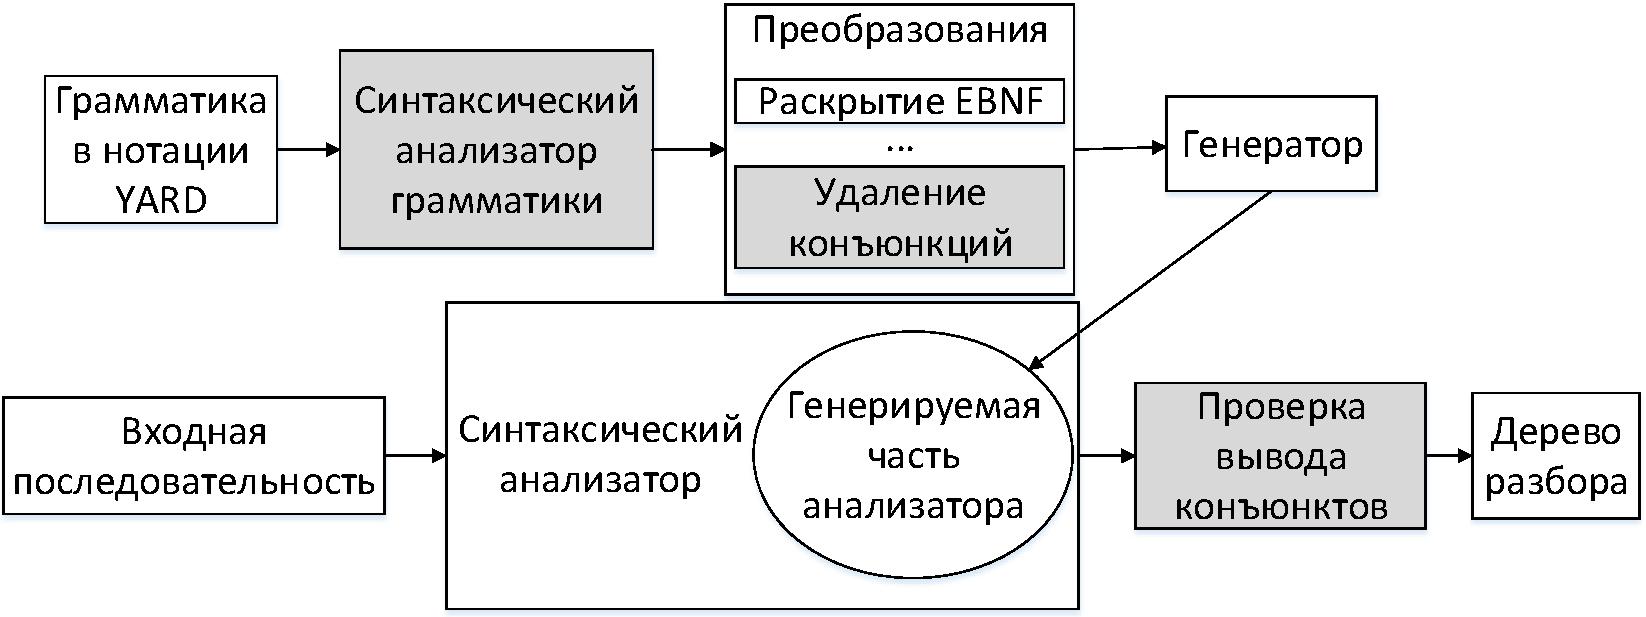
\includegraphics[width=16cm]{courseworkpictures/img3.pdf}
\caption{Структура решения с учётом внесённых изменений}
\label{Структура_с_учётом_внесённых_изменений}
\end{figure}

\section{Эксперименты}

Были проведены экспериментальные исследования, целью которых являлась проверка того, что конъюнктивные грамматики позволяют задавать структуру тРНК так, что синтаксический анализатор находит меньше некорректных цепочек.

\begin{figure}[h]
\begin{center}
\begin{verbatim}

[<Start>]
folded: stem<(any*[1..3] 
              stem<any*[7..10]> 
              any*[1..3] 
              stem<any*[5..8]> 
              any*[3..5] 
              stem<any*[5..8]>
              )>

stem<s>: 
      A stem<s> U
    | U stem<s> A
    | C stem<s> G
    | G stem<s> C
    | G stem<s> U
    | U stem<s> G
    | s

any: A | U | G | C

\end{verbatim}
\caption{КС-грамматика вторичной структуры тРНК}
\label{TRNAgrammar}
\end{center}
\end{figure}

\begin{figure}
\begin{center}
\begin{verbatim}
[<Start>]
folded: stem<subseq> & (any*[7..9] subseq any*[7..9])

subseq: any*[1..3] 
        stem<any*[7..10]> & (any*[4..6] any*[7..10] any*[4..6])
        any*[1..3] 
        stem<any*[5..8]> & (any*[6] any*[5..8] any*[6])
        any*[3..5] 
        stem<any*[5..8]> & (any*[4..5] any*[5..8] any*[4..5])
        
stem<s>:
      A stem<s> U
    | U stem<s> A
    | C stem<s> G
    | G stem<s> C
    | G stem<s> U
    | U stem<s> G
    | s

any: A | U | G | C

\end{verbatim}
\caption{Конъюнктивная грамматика структуры тРНК}
\label{TRNAgrammarConj}
\end{center}
\end{figure}


\begin{figure}
\begin{center}
\begin{tikzpicture}
\begin{axis}[
    legend pos = north west,
  xlabel = {Количество лексем},
  ylabel = {Время, с}
]
\addplot coordinates {
  (100,2) (200,17) (300,42) (400,81) (500,128) (600,190) (700,264) (800,345) (900,446) (1000,562)
};
\addplot coordinates {
  (100,1) (200,2) (300,4) (400,8) (500,12) (600,18) (700,22) (800,28) (900,36) (1000,43)
};
\legend{ 
  грамматика $G_{2}$, 
  грамматика $G_{3}$
};
\end{axis}
\end{tikzpicture}
\end{center}
\caption{Среднее время работы алгоритма на конъюнктивной и контекстно-свободной грамматиках тРНК}
\label{time}
\end{figure}

\begin{table}[h]
\begin{center}
  \begin{tabular}{ | c | c | c |}
    \hline
     & КС-грамматика & Конъюнктивная грамматика \\ \hline
    Тест 1. Кол-во ошибок: & 15 & 0 \\\hline
    Тест 2. Кол-во ошибок: & 5 & 0 \\\hline
    Тест 3. Кол-во ошибок: & 11 & 0 \\
    \hline
  \end{tabular}
\end{center}
\caption{Количество некорректных цепочек, распознанных синтаксическим анализатором}
\label{mistakes}
\end{table}

На рисунках~\ref{TRNAgrammar} и~\ref{TRNAgrammarConj} представлены грамматки, описывающие структуру тРНК. Грамматика $G_2$ является контекстно-свободной, а грамматика $G_3$ --- конъюнктивной. По данным грамматикам были сгенерированы соответствующие синтаксические анализаторы.

На вход построенным синтаксическим анализаторам подавались сгенерированные цепочки ДНК длиной от 100 до 1000 симовлов. Эти цепочки содержали в себе последовательности тРНК, а также другие последовательности, которые можно ложно признать за тРНК. Напимер, цепочка на рисунке~\ref{rnachain}, хоть и не является тРНК, распознаётся грамматикой $G_2$, но не распознаётся грамматикой $G_3$.

\begin{figure}
\begin{center}
ACACCCCCCCUCACCCCCUCCCACCCCCUU
\end{center}
\caption{Пример цепочки нуклеотидов, сгенеированной для экспериментов}
\label{rnachain}
\end{figure}


Результаты экспериментов приведены в таблице~\ref{mistakes}. Из них ясно, что грамматика $G_2$ не распознаёт ложные цепочки, распознавыемые грамматикой $G_3$. Время работы синтаксических анализаторов показано на графике, изображённом на рисунке~\ref{time}. По графику видно, что время работы синтаксического анализатора, построенного по грамматике $G_3$, значительно превышает время работы другого.

Таким образом, конъюнктивная грамматика позволяет отсеивать цепочки, ложно распозначаемые КС-грамматикой, но за время, значительно большее, чем время работы анализатора по КС-грамматике.






% У заключения нет номера главы
\section*{Заключение}
В ходе работы получены следующие результаты:
\begin{itemize}
    \item реализована поддержка конъюнктивных грамматик в языке спецификации грамматик YARD;
    \item реализована поддержка конъюнктивных грамматик в генераторе GLL-анализаторов;
    \item результаты экспериментально проверены на небольших метагеномных сборках.
\end{itemize}

\subsubsection*{Дальнейшее направление работ}

В первую очередь, необходимо снизить время работы алгоритма. Полученная реализация предполагает полный обход дерева разбора, что, безусловно, влияет на производительность алгоритма. Кроме того, можно исследовать возможность расширения класса распознаваемых языков до булевых, на основе полученных результатов.

\setmonofont[Mapping=tex-text]{CMU Typewriter Text}
\bibliographystyle{ugost2008ls}
\bibliography{diploma.bib}
\end{document}
